\subsection{Model Dynamics}
\label{sec:state.og.dynamics}

We are interested in the dynamics \hl{of the original model with fixed} parameters $\beta = 1, f = 150, L = 4.2 \cdot 10^{-3}, R = 2, V_m = 5,$ and $\mu = 0.5$.
The parameters $E_0$ and $\chi_0$ are varied in the ranges $[14, 28]$ and $[0.1, 0.65]$, respectively.
Scanning this parameter plane for the period of stable cycles results in \Cref{fig:setup.og.dynamics.period}.

\begin{figure}
	\centering
	\includegraphics[width=0.6\textwidth]{99_Yunus/2D_Period_Zoomed/result.png}
	\caption[2D scan of the periods in the original model]{
		2D scan of the periods in the original model.
		The parameters $\beta = 1, f = 150, L = 4.2 \cdot 10^{-3}, R = 2, V_m = 5,$ and $\mu = 0.5$ are fixed.
		The parameters $E_0$ and $\chi_0$ are varied in the ranges $[14, 28]$ and $[0.1, 0.65]$, respectively.
	}
	\label{fig:setup.og.dynamics.period}
\end{figure}

\hl{
	The colors in the 2D scan \Cref{fig:setup.og.dynamics.period} indicate the period of the stable cycle in those regions.
	Brighter colors mean higher periods.
}
Points $A, B$ and $C$ are in the parameter region, which has stable cycles with the period 12.
The period regions, in which these points are, differ in another way.
Besides the period of a cycle, there is another characteristic, the symbolic sequence.
As mentioned before, it describes on which branches of the model function the points of the cycle exist.
Some \hl{cobweb diagrams} illustrate the difference between the parameter regions.

\Cref{fig:yunus.2pi.CobwebA12,fig:yunus.2pi.CobwebC12} show the \hl{cobweb diagrams} at points $A$ and $C$.
Both parameter regions have only one stable cycle of period 12.
The stable cycle at point $A$ has the symbolic sequence $\A^3\B^3\C^3\D^3$ and the cycle at point $C$ has the symbolic sequence $\A^2\B^4\C^2\D^4$.
We follow the convention, that the branch with the smallest positive boundaries is called branch $\A$.
\hl{And the next one branch $\B$ and so on.}
\hl{
	The cycles at point $A$ and point $C$ are symmetrical.
	This is due to an inherit symmetry in the model.
	\Cref{equ:state.os.sym} describes this symmetry.
	It means, that the model behaves the same on its left half $[0, \pi]$ as it does on its right half $[\pi, 2\pi]$.
	This is important to understand the cycles at point $B$ better.
}

\begin{align}
	F(\theta + \pi) \equiv F(\theta) + \pi \mod 2\pi \label{equ:state.os.sym}
\end{align}

\Cref{fig:yunus.2pi.CobwebB12} shows the \hl{cobweb diagram} at point $B$.
\hl{By looking closely, one can see that there are 2 coexisting cycles in this cobweb diagram.}
One cycle has the symbolic sequence $\A^3\B^3\C^2\D^4$, while the other one has the symbolic sequence $\A^2\B^2\C^3\D^3$.
\hl{
	Both cycles are asymmetric.
	And they are similar to each other in the way that $\Cycle{\A^3\B^3\C^2\D^4}$ behaves on the branches $\A$ and $\B$ like $\Cycle{\A^2\B^2\C^3\D^3}$ on the branches $\C$ and $\D$ and vice versa.
	One can think of the cycles being equivalent by shifting them by $\pi$ in either direction.
	Due to the symmetry of the model, an asymmetric stable cycle necessarily must exist alongside another asymmetric stable cycle that is itself, but shifted by $\pi$.
	These cycles also behave similarly to both the cycles at points $A$ and $B$.
}
The cycle $\Cycle{\A^3\B^3\C^2\D^4}$ behaves like the cycle $\Cycle{\A^3\B^3\C^3\D^3}$ at point $A$ on its left half, while it behaves like the cycle $\Cycle{\A^2\B^4\C^2\D^4}$ on its right half.
The same is true for the cycle $\Cycle{\A^2\B^4\C^3\D^3}$ but reversed since it is the other cycle \hl{shifted} by $\pi$.
\hl{
	We call the previously described parameter regions with only one symmetrical stable cycle ``type A'' parameter regions.
	The just described parameter regions with 2 asymmetrical coexisting cycles will be called ``type B'' parameter regions.
}

\begin{figure}
	\centering
	\begin{subfigure}{0.3\textwidth}
		\centering
		\includegraphics[width=\textwidth]{99_Yunus/Period12/Cobweb_A_12/result.png}
		\caption{At Point $A$}
		\label{fig:yunus.2pi.CobwebA12}
	\end{subfigure}
	\begin{subfigure}{0.3\textwidth}
		\centering
		\includegraphics[width=\textwidth]{99_Yunus/Period12/Cobweb_B_12/result.png}
		\caption{At Point $B$}
		\label{fig:yunus.2pi.CobwebB12}
	\end{subfigure}
	\begin{subfigure}{0.3\textwidth}
		\centering
		\includegraphics[width=\textwidth]{99_Yunus/Period12/Cobweb_C_12/result.png}
		\caption{At Point $C$}
		\label{fig:yunus.2pi.CobwebC12}
	\end{subfigure}
	\caption[Cobweb diagrams of the original model]{
		Cobweb diagrams at three values of the parameters $E_0$ and $\chi_0$ in the original model with fixed parameters $\beta = 1, f = 150, L = 4.2 \cdot 10^{-3}, R = 2, V_m = 5,$ and $\mu = 0.5$.
		The parameter values of $E_0$ and $\chi_0$ are marked in \Cref{fig:setup.og.dynamics.period}.
	}
\end{figure}

This behavior is peculiar.
To summarize, we have chains of parameter regions with the same period.
The type of the parameter regions alternates between ``type A'' and ``type B''.
When the stable cycle in one ``type A'' parameter region is $\Cycle{\A^x\B^y\C^x\D^y}$, the stable cycle in the next ``type A'' parameter region is $\Cycle{\A^{x-1}\B^{y+1}\C^{x-1}\D^{y+1}}$.
The ``type B'' parameter region in between two ``type A'' parameter regions of a chain with cycles $\Cycle{\A^x\B^y\C^x\D^y}$ and $\Cycle{\A^{x-1}\B^{y+1}\C^{x-1}\D^{y+1}}$, has the two cycles $\Cycle{\A^x\B^y\C^{x-1}\D^{y+1}}$ and $\Cycle{\A^{x-1}\B^{y+1}\C^x\D^y}$.
Also, there is not only one chain, but many chains next to each other where the period increases by 2 from one chain to the next.
